\documentclass[tikz,border=10pt,dvipsnames]{standalone}
\usetikzlibrary{
  arrows.meta,                        % for arrow tips
  backgrounds,                        % for background layer
  bending,
  ext.paths.ortho,                    % for ortho paths
  positioning,
  ext.positioning-plus,               % for 
  ext.node-families.shapes.geometric, % loads ext.node-families and
% shapes.geometric,                   % for ellipse
  calc,                               % for ($$)
  backgrounds %https://tex.stackexchange.com/questions/230224/how-to-change-the-background-color-in-tikz
}
% node styles
\tikzstyle{flowstep} = [rectangle, draw, text centered, rounded corners, minimum height=2em]
\tikzstyle{concept}=[flowstep,fill=orange!20]
\tikzstyle{simstep}=[flowstep,fill=yellow!20]
\tikzstyle{veristep}=[flowstep,fill=BurntOrange!60]
\tikzstyle{designstep}=[flowstep,fill=pink!50]
\tikzstyle{expensivestep}=[flowstep,fill=red!30]
% edge styles
\tikzstyle{happypath}=[->,rounded corners,thick,ForestGreen!75!white]
% no arrow
\tikzstyle{unhappypathna}=[rounded corners,thick,BrickRed!75!white]
\tikzstyle{unhappypath}=[->,unhappypathna]
\tikzstyle{veryunhappypath}=[rounded corners,thick,Red,->]
\tikzset{
  fill fraction/.style n args={3}{path picture={
 \fill[#1] (path picture bounding box.south west) rectangle
 ($(path picture bounding box.north west)!#3!(path picture bounding box.north
 east)$);
 \fill[#2] (path picture bounding box.south east) rectangle
 ($(path picture bounding box.north west)!#3!(path picture bounding box.north
 east)$);}}
}

\begin{document}
%source: andreas burg https://ee222-winter19-01.courses.soe.ucsc.edu/system/files/attachments/EE222W19_Lect1_Part2-Introduction.pdf

% TODO add an image to each level, unveil in 2nd step all at once
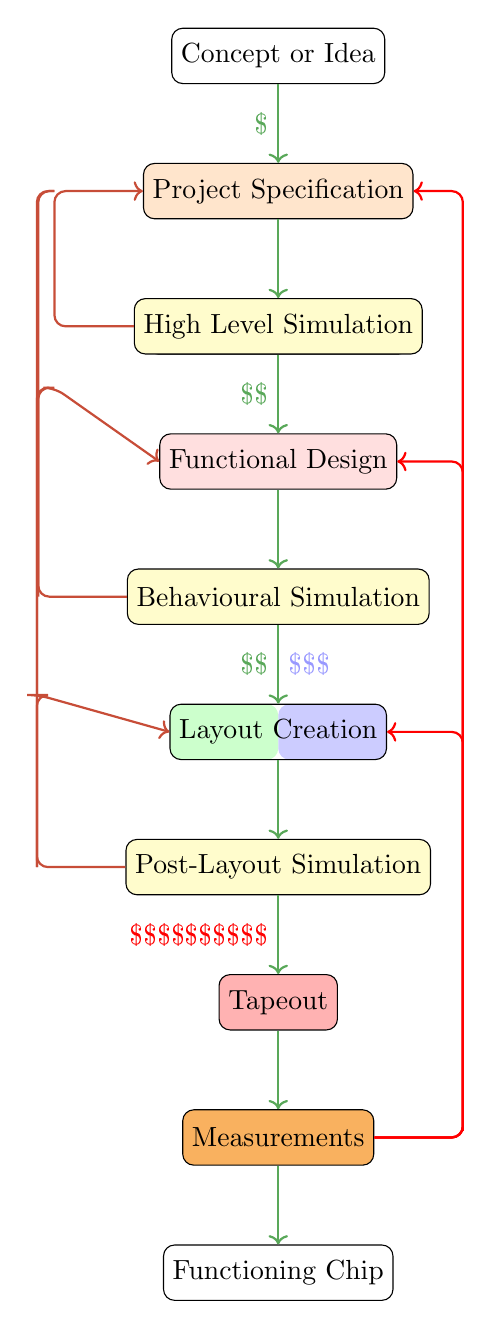
\begin{tikzpicture}
  % first flow nodes
\node[flowstep](conceptidea) at (3,0) {Concept or Idea};
\node[concept](projspec)[below=of conceptidea]{Project Specification};
\node[designstep](archstep)[below=of projspec]{Architectural design}; % high level specification,break into logical blocks
\node[simstep](highsimulation)[below=of projspec]{High Level Simulation}; % often adhoc
\node[designstep](schematic)[below=of highsimulation]{Functional Design}; %Schematic
\node[simstep](simulation)[below=of schematic]{Behavioural Simulation}; % VHDL model
\node[flowstep,fill fraction={green!20}{blue!20}{0.5}](layout)[below=of simulation]{Layout Creation}; % can either be full custom or semi custom, will involve netlist,floor plan place and route
\node[simstep](postsim)[below=of layout]{Post-Layout Simulation}; % VHDL model
\node[expensivestep](tapeout)[below=of postsim]{Tapeout}; % VHDL model
\node[veristep](physmeas)[below=of tapeout]{Measurements}; % VHDL model
\node[flowstep](chip) [below=of physmeas] {Functioning Chip};

% now happy path
\draw[happypath](conceptidea) -- (projspec) node [midway,left]{\$};
\draw[happypath](projspec) -- (highsimulation);
\draw[happypath](highsimulation) -- (schematic) node [midway,left]{\$\$};
\draw[happypath](schematic) edge (simulation);
\draw[happypath](simulation) -- (layout) node [midway, left]{\$\$} node [midway, right,color=blue!40]{\$\$\$};
\draw[happypath](layout) edge (postsim);
\draw[happypath](postsim) -- (tapeout) node [midway,left,color=red]{\$\$\$\$\$\$\$\$\$\$};
\draw[happypath](tapeout) edge (physmeas);
\draw[happypath](physmeas) edge (chip);
% unhappy path
% control points for  cleaner paths
\node (ctrlPS) [left=of projspec] {};
\node (ctrlHS) [left=of highsimulation.west,below=of ctrlPS] {};
\draw[unhappypath] (highsimulation.west) -| (ctrlHS.center) -- (ctrlPS.center) -> (projspec.west);
\node (ctrlFD) [left=of schematic,below=of ctrlHS] {};
\node (ctrlBS) [below=of ctrlFD,left=of simulation] {};
\draw[unhappypath] (simulation.west) -| (ctrlBS.center) |- (ctrlFD.center) -> (schematic.west);
\draw[unhappypathna] (ctrlBS.center) |- (ctrlPS.center);
\node (ctrlLG) [left=of layout,below=of ctrlBS] {};
\node (ctrlPLS) [below=of ctrlLG,left=of postsim] {};
\draw[unhappypath] (postsim.west) -| (ctrlPLS.center) |- (ctrlLG.center) -> (layout.west);
\draw[unhappypathna] (ctrlPLS.center) |- (ctrlFD.center);
\draw[unhappypathna] (ctrlPLS.center) |- (ctrlPS.center);
\node (ctrlTO) [right=of tapeout] {};
\node (ctrlMeas) [below=of ctrlTO,right=of physmeas] {};
\draw[veryunhappypath] (physmeas.east) -|(ctrlMeas.center) |- (layout.east);
\draw[veryunhappypath] (physmeas.east) -|(ctrlMeas.center) |- (schematic.east);
\draw[veryunhappypath] (physmeas.east) -|(ctrlMeas.center) |- (projspec.east);

% *very* unhappy paths
\end{tikzpicture}
\end{document}
